\chapter{InstaGame}\label{chap:method}

% Introduction to the tool
\section{Introduction}

The proposed tool, InstaGame, is designed to address key limitations identified in existing educational game creation platforms, such as SGAME \cite{sgame2020}. While SGAME enables educators to integrate SCORM-compliant learning objects into preexisting game templates, it restricts flexibility in game creation, limits educational content to the Spanish language, and primarily caters to middle school to high school curricula. In contrast, InstaGame empowers instructors to create highly customizable games tailored to diverse educational contexts and languages. By decoupling game templates from specific fields, the tool fosters inclusivity and usability while accommodating a wide range of educational levels and subjects.

% explain the design and architecture of the tool
\section{Design and Architecture}

To ensure accessibility across devices and platforms, InstaGame adopts a web-based architecture. Instructors use a portal to design games and share them with students via links, QR codes, or game codes, making them accessible on any device with a web browser. The backend leverages Firebase as a Backend as a Service (BaaS) to store game data in the cloud, ensuring global availability. However, due to changes in Firebase's pricing policy, Appwrite, an open-source service, was integrated as an alternative storage solution.

The instructor portal is developed using Next.js, a React framework that supports server-side rendering, while the game templates include a Space Invaders-like game developed in Unity and hosted on itch.io, as well as a click-based puzzle game created with Next.js. These templates are highly adaptable, enabling instructors to incorporate educational content specific to their needs. The system architecture is depicted in Figure \ref{fig:architecture}.

\begin{figure}
	\centering
	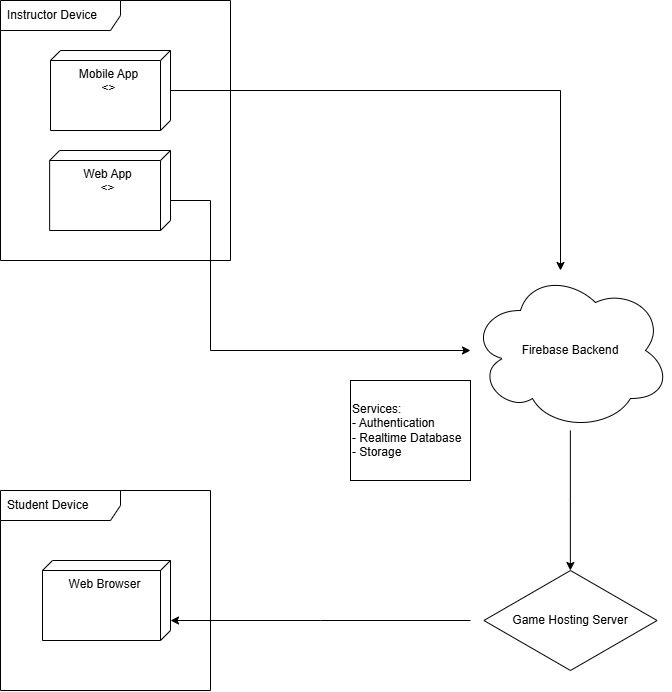
\includegraphics[width=0.8\textwidth]{figures/Deployment_UML.jpg}
	\caption{System Architecture}
	\label{fig:architecture}
\end{figure}

% explain the levling system behind the tool
\section{Leveling System}

InstaGame incorporates a leveling system to maintain student engagement and provide a structured learning experience. For instance, in the Space Invaders-like game template, players must complete levels by answering educational questions correctly. Each level consists of an odd number of challenges or turns, and players must achieve more than half correct answers to advance. For example, a level with five challenges requires at least three correct answers for progression.

The interface displays relevant information such as the current turn, level, challenge text, and goal. Interactive elements, including "Submit" and "Reset" buttons, allow players to confirm their choices or correct input errors. This system ensures that students are consistently challenged while reinforcing their understanding of the subject matter.

% explain the goal checking system behind the tool
\section{Goal Checking System}

The goal-checking system in InstaGame ensures alignment between gameplay and educational objectives. In the Space Invaders-like game, each enemy represents a potential answer to an educational question. Players must destroy enemies corresponding to the correct answers to progress through the game. Similarly, in the click-based puzzle game, players interact with images to select the correct answers, such as diagnosing a disease by clicking on the affected organ.

Instructors define the goals and criteria for success when creating games. For example, in the puzzle game, instructors upload images, mark clickable regions, and provide contextual information, such as dialogues describing symptoms or conditions. The system evaluates player actions against these predefined goals to determine success, offering immediate feedback to enhance the learning experience.

% explain the game sharing system being used in the tool
\section{Game Sharing System}

InstaGame simplifies the process of sharing games with students through its game sharing system. Once a game is created using the instructor portal, a link, QR code, and game code are generated automatically. These sharing options enable students to access the game seamlessly on their preferred devices.

For games requiring additional assets, such as images for the click-based puzzle game, instructors upload the necessary files to Firebase Storage or Appwrite during game creation. This ensures that all required resources are readily available to students upon accessing the game. By streamlining the sharing process, InstaGame enhances accessibility and fosters collaboration between instructors and students.

